\documentclass[a4paper,12pt]{article}

%\documentclass[11pt,a4paper,oneside]{report}
\usepackage[top=0.75in, bottom=0.75in, left=1.25in, right=0.75in]{geometry}
\usepackage[pdftex]{graphicx}
\usepackage[T1]{fontenc}
\usepackage{fancyhdr}
\usepackage{algorithm}
\usepackage{algorithmic}
\usepackage{amssymb}
\usepackage{amsmath}
\usepackage{subfigure}
\setcounter{tocdepth}{3}
\usepackage{graphicx}
\usepackage{enumerate}
\usepackage{verbatim}

\newcommand{\HRule}{\rule{\linewidth}{0.5mm}}

\makeatletter
\newcommand{\rmnum}[1]{\romannumeral #1}
\newcommand{\Rmnum}[1]{\expandafter\@slowromancap\romannumeral #1@}
\makeatother

\begin{document}

\renewcommand*\rmdefault{ppl}\normalfont\upshape
\renewcommand{\headrulewidth}{0.5pt}
\renewcommand{\footrulewidth}{0.5pt}

%\pagestyle{fancy}

%%%%%%%%%%%%%%%%%%%%%%%%%%%%%%%%%%%%%%%%%%%%%%%%%%%%TITLE PAGE%%%%%%%%%%%%%%%%%%%%%%%%%%%%%%%%%%%%%%%%%%%%%%%%%%%%%%%%%%%%%%%%%%%%%%%%%%%

\begin{titlepage}
\begin{center}
\newpage


\includegraphics[width=0.3\textwidth]{./logo}\\[2cm]    
%\textsc{\LARGE PES Institute of Technology}\\[1.5cm]

\textsc{\Large  \Rmnum{6} Semester Special Topic}\\[0.5cm]

\HRule \\[0.4cm]
{ \huge \bfseries A Bidirectional Search Algorithm in Power Law Networks}\\[0.4cm]
\HRule \\[1.5cm]

\vspace{1in}
% Title

% Author and supervisor
\begin{minipage}{0.4\textwidth}
\begin{flushleft} \large
\emph{By:}\\
Vijay Mahantesh S M\\
-1PI09CS118\\
Vijesh M\\
-1PI09CS119
\end{flushleft}
\end{minipage}
\begin{minipage}{0.4\textwidth}
\begin{flushright} \large
\emph{Guided By:} \\
Dr. Kavi Mahesh\\
Professor \\
Computer Science Dept\\
PESIT, Bangalore 
\end{flushright}
\end{minipage}

%\vfill
% Bottom of the page
\end{center}
\end{titlepage}
%%%%%%%%%%%%%%%%%%%%%%%%%%%%%%%%%%%%%%%%%%%%%%%%%%%%END TITLE PAGE%%%%%%%%%%%%%%%%%%%%%%%%%%%%%%%%%%%%%%%%%%%%%%%%%%%%%%%%%%%%%%%%%%%%%%
\begin{center}

\vspace{15in}


\includegraphics[width=0.3\textwidth]{./logo}\\[2cm]    

\includegraphics[width=0.3\textwidth]{./certificate-text.png}\\[2cm]
\normalfont
\rmfamily{\Large{This is to certify that Vijay Mahantesh SM (1PI09CS118) and Vijesh M (1PI09CS119) have satisfactorily completed the Special Topic Project prescribed by PES Institute of Technology (Autonomous Institute under VTU) in the year 2012 (January - May).}}\\[4cm]
\begin{minipage}{0.4\textwidth}
\begin{flushleft} \large
\emph{Signature of Guide}\\
Dr. Kavi Mahesh
\end{flushleft}
\end{minipage}
\begin{minipage}{0.4\textwidth}
\begin{flushright} \large
\emph{Signature of HOD} \\
Prof. Nitin V Pujari 
\end{flushright}
\end{minipage}
\end{center}



\newpage
\section*{\Huge{Acknowledgment}}
We wish to express our sincere gratitude to Nitin V Pujari, HOD, Computer Science Department, PESIT for providing us with an opportunity to carry out the special topic on ''A Bidirectional Search Algorithm in Power Law Networks''. We also wish to express our gratitude to Dr. Kavi Mahesh, Computer Science Department, PESIT for providing us with the guidance needed. We would like to thank Prof. C Pandu Rangan, IIT, Chennai, India, for providing us an opportunity to intern at IIT Chennai during June-July 2011. We would also like to thank Dr. Sudarshan Iyengar, ISI, Chennai, India, for providing us with a strong foundation of the basic concepts required and his invaluable guidance.

\newpage
\section*{\Huge{Abstract}}
Searching in networks is one of the most frequently stumbled upon requirements in network analysis. Most of the Real World networks, such as computer networks and social networks, exhibit a power law degree distribution. The high connectivity nodes play the important role of hubs in communication and networking. This fact is exploited when designing efficient local search algorithms. Lada A. Adamic introduces one such searching strategy in the paper titled "Search in Power-Law Networks". The idea proposed in the paper involves a unidirectional search technique, wherein the search is initiated from the source node and ends at the destination node. Our idea is an extension of the idea proposed in the paper. Instead of a unidirectional search, we use a bidirectional technique. We demonstrate the performance of this technique on synthetic scale-free networks and gnutella peer-to-peer networks.
\newpage

\newpage
\tableofcontents

%\pagestyle{fancy}
%\renewcommand{\chaptermark}[1]{\markboth{#1}{}}


\cfoot{\thepage}

\newpage
\section{Problem Definition}
We frequently stumble upon applications that requires finding the shortest path between various nodes in a network. From ages, many algorithms have been proposed to solve this problem. One such is algorithm is Dijkstra's single source shortest path algorithm. The complexity involved in finding all pair shortest path in a network of $n$ nodes, using this algorithm is $O(n^3)$. Some applications just require a path establishment between a given pair of nodes. There might not exist a hardbound constraint that the established path must be the shortest. In such a case, Dijkstra's algorithm creates an extra overhead of computing the exact shortest path. The technique proposed by Adamic aims to solve this problem, but with the path length tradeoff. Here we focus on finding an approximate shortest path between any two nodes by tweaking Adamic's unidirectional search algorithm.

\section{Introduction}
The problem of finding a target vertex in a network where one is provided with just the local information is a well studied problem. Starting from the work of Milgram in 1967~\cite{milgram67}, the current methods include routing using full-tables~\cite{gavoille01}, interval routing~\cite{gavoille99,gavoille01}, routing labeling schemes~\cite{peleg00,thorup01}, greedy routing~\cite{giordano01,kleinberg-1-00}, geographic routing~\cite{giordano01}, compass routing~\cite{giordano01}, 
etc., These routing techniques are mainly used in transportation networks and in wired as well as wireless communication networks. For detailed survey one can refer to~\cite{gavoille99, gavoille01, giordano01} and~\cite{peleg00}. For surveys of the routing methods in social networks and email networks in particular, one is referred to~\cite{adamic02, adamic01, fraigniaud07, kleinberg-1-00, nowell05} 


%
%(adamic02)[3]
%(adamic01)[4]
%(fraigniaud07)[33]
%(gavoille99)[37]
%(gavoille01)[38]
%(giordano01)[43]$\frac{length of actual path}{length of shortest path}$
%(kleinberg-1-00)[47]
%(nowell05)[54]
%(peleg00)[56]
%(thorup01)[65]
 
In the classical small world experiment by Milgram~\cite{milgram67}, the letter from Nebraska was to reach Boston. This is a scenario where the sender actively needs to participate in the process of helping the letter reach the destination, while the receiver remains passive. Let us consider a variation of this problem where both sender and receiver participate in the process of finding a path between them. 

\subsection{Motivation}

The motivation for the extension of Adamic's algorithm arises from the intuition that the network navigation can be performed in a more efficient way by considering bidirectional search. The underlying network is not visible to the walkers in its entirety. At any instance, the walkers can view the adjacent nodes of the node that it is currently present. During the analysis phase, several such source-destination node pairs are given to the walkers. The time taken and the path taken are recorded.\\

In the current study, we present a \emph{navigation algorithm} that combines Adamic's navigation technique and one of the strategy used by human participants in the experiment reported in \cite{sudarshan11}. 

\subsection{The Technique}
In an unweighted graph $G(V,E)$, given a source vertex $s$ and a destination vertex $t$, a straightforward approach to establish a path between $s$ and $t$ is to take a random walk from $s$ till we reach $t$. One way to better this random walk method is to take a two way random walk, one from the source $s$ and the other from the destination $t$ and stop once the two random walks intersect. This method is expected to be quicker than the first in terms of number of hops that is required to establish a path. We provide empirical results to support this.\\

This is a generic algorithm that can be applied on any type of network. Hence, it doesn't exploit the underlying structure of the network and its characteristics. Adamic's greedy walk algorithm exploits the characteristics of the power law network. We describe an extension of the algorithm that involves bidirectional search.

\section{Literature Survey}
\label{sec:4_related_work}
Kleinberg's work~\cite{kleinberg-2-00} on navigation in a small world, was the first paper to shed light on the navigation problem on complex networks. The paper highlighted the fact that it is easier to find short chains between points in \emph{some} networks than \emph{others}.\\

Adamic et al., in~\cite{adamic01} introduced several local search strategies to find a path to the given destination vertex. Their strategies are limited to applications on networks that obey the power law. The results are shown on gnutella peer-to-peer network which is known to obey power law. In~\cite{kim02}, Kim et al., numerically compares the local path finding strategies with that of global path finding strategies on scale free networks.\\ 

Adamic et al., in~\cite{adamic05} addresses the question of how participants in a small world experiment are able to find short paths in a social network using only local information about their immediate contacts. They conduct their experiment on an email network and demonstrate by empirical data that the small world search strategies using a contact's position in physical space or in an organizational hierarchy relative to the target can effectively be used to locate most individuals.\\

A detailed survey on decentralized search algorithms on networks that exhibit small-world phenomena is given by Kleinberg in~\cite{kleinberg06}. This survey also contains an exhaustive list of open problems in this area.\\

On the application front, such navigational techniques are useful in a problem of finding paths between vertices in peer-to-peer systems.  Crespo et al.,~\cite{crespo02} in their work on routing indices on Peer-to-Peer systems, propose a novel method of query forwarding from vertices to their neighbors that are more likely to have answers. They provide different novel routing schemes and evaluate their performance.

\newpage
\section{The Algorithm}
\label{sec:idea}
Adamic's search technique involves the initiation of the search from the source. The walker, initially placed at the source, hops to that neighbor with the highest degree. The walker then checks to see if the destination is reached. If the walker hasnt reached the destination, a simlar action is performed from the current node. The algorithm terminates if the walker has reached the destination. A potential problem that could arise from this algorithm is the formation of cycles. According the technique, if the next hop tends to form a cycle, the neighbor with the next highest degree is chosen.

The Bidirectional Search Algorithm functions on similar lines, but with a tweak. It can be split into two parallelizable components.

\begin{itemize}
\item Search from the source
\item Search from the destination
\end{itemize}

The logic for individual searches from either the source or the destination is same as that of Adamic's technique. At every time step, both the walkers advance one step in the manner described above. After each advancement, we check whether there is an intersection of the paths traced. When an intersection occurs, we note the time taken and the paths traversed.\\

In our experiments that follow, we show the results of application of our algorithm on classes of graphs such as Barabasi Albert Networks, Erdos Renyi Networks and Gnutella peer-to-peer network.

\subsection{Comparison Between Various Navigation Techniques}

This section highlights the effectiveness of greedy navigation over other methods of navigation. Consider two vertices $s,t \in V$. Let $s$ be source and $t$ be the target vertex. In the navigation phase of the algorithm, our aim is to establish a path between $s$ and 
$t$. Let $d(s,t)$ denote the length of the shortest path between $s$ and $t$. Here are a few methods one can adopt to accomplish the task of establishing a path between $s$ and $t$:

\subsubsection {1-Way Random Walk}
The idea here is to start from the source vertex $s$ and take a random walk 
$W_s$ until the target vertex $t$ is reached. Since this technique involves 
a single random walk, we refer to it as a 1-way random walk. Let 
$\beta_{s,t}$ denote the path length of the path corresponding to the random 
walk $W_s$ from $s$ to $t$. Let $\beta$ be the 
average ratio of length of 1-way random walk and length of the shortest 
path, taken over all unordered vertex pairs $(s,t)$, such that $s,t \in V$.
$$\beta = \frac{1}{\left(\begin{array}{c} |V|\\ 2\end{array}\right)} \sum_{s,t \in V} 
\frac{\beta_{s,t}}{d(s,t)}$$	

Figure.~\ref{4_one_way} illustrates the technique of 1-way random walk from $s$ to $t$. $W_s$
terminates when it reaches $t$. $W_s$ is indicated by the red walk. The source $s$ 
and target $t$ is denoted by the red dots. The blue dots indicate the other vertices 
in the network. 

\begin{figure}[htp]
\centering
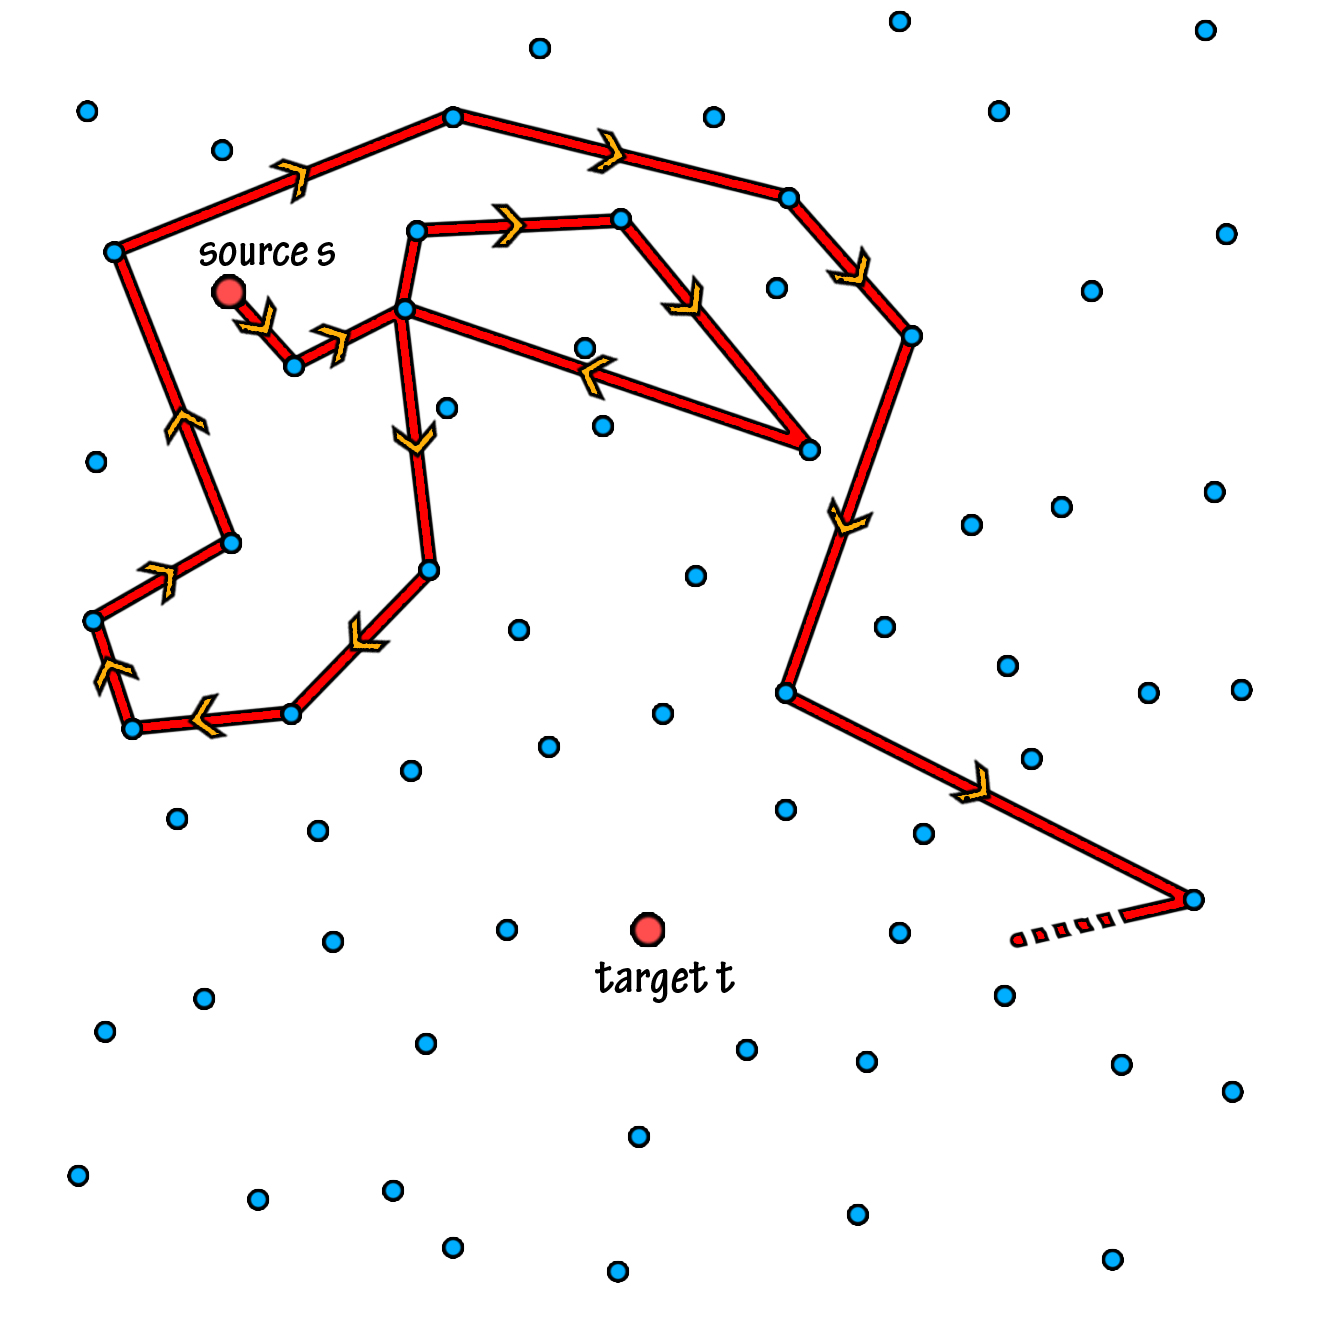
\includegraphics[scale=0.14]{Results/1rawrandomwalk.jpg}
\caption{1-way Random Walk}
\label{4_one_way}
\end{figure}

\subsubsection{2-Way Random Walk}

After taking random walks $W_s$ and $W_t$ from $s$ and $t$ simultaneously 
until the two walks intersect, one can find a path from $s$ to $t$.

This idea is similar to the one implemented in the learning phase in 
Section ~\ref{sec:4_learning_phase}. Let $\gamma_{s,t}$ denote the length of the path thus obtained. 
Let $\gamma$ be the average ratio of length of 2-way Random Walk and the 
length of the shortest path taken over all the unordered vertex pairs $(s,t)$, such that $s,t \in V$.


$$\gamma = \frac{1}{\left(\begin{array}{c} |V|\\ 2\end{array}\right)} \sum_{s,t \in V} \frac{\gamma_{s,t}}{d(s,t)}$$

Figure~\ref{4_two_way} illustrates the technique of 2-way random walk between $s$ and $t$. 
$W_s$ and $W_t$ are constructed simultaneously until they intersect.
The intersection point of the two walks is indicated by $H$. $W_s$ and $W_t$ 
are indicated by the red walk and green walk respectively. Source $s$ and the 
target $t$ are denoted by the red dots. 

\begin{figure}[htp]
\centering
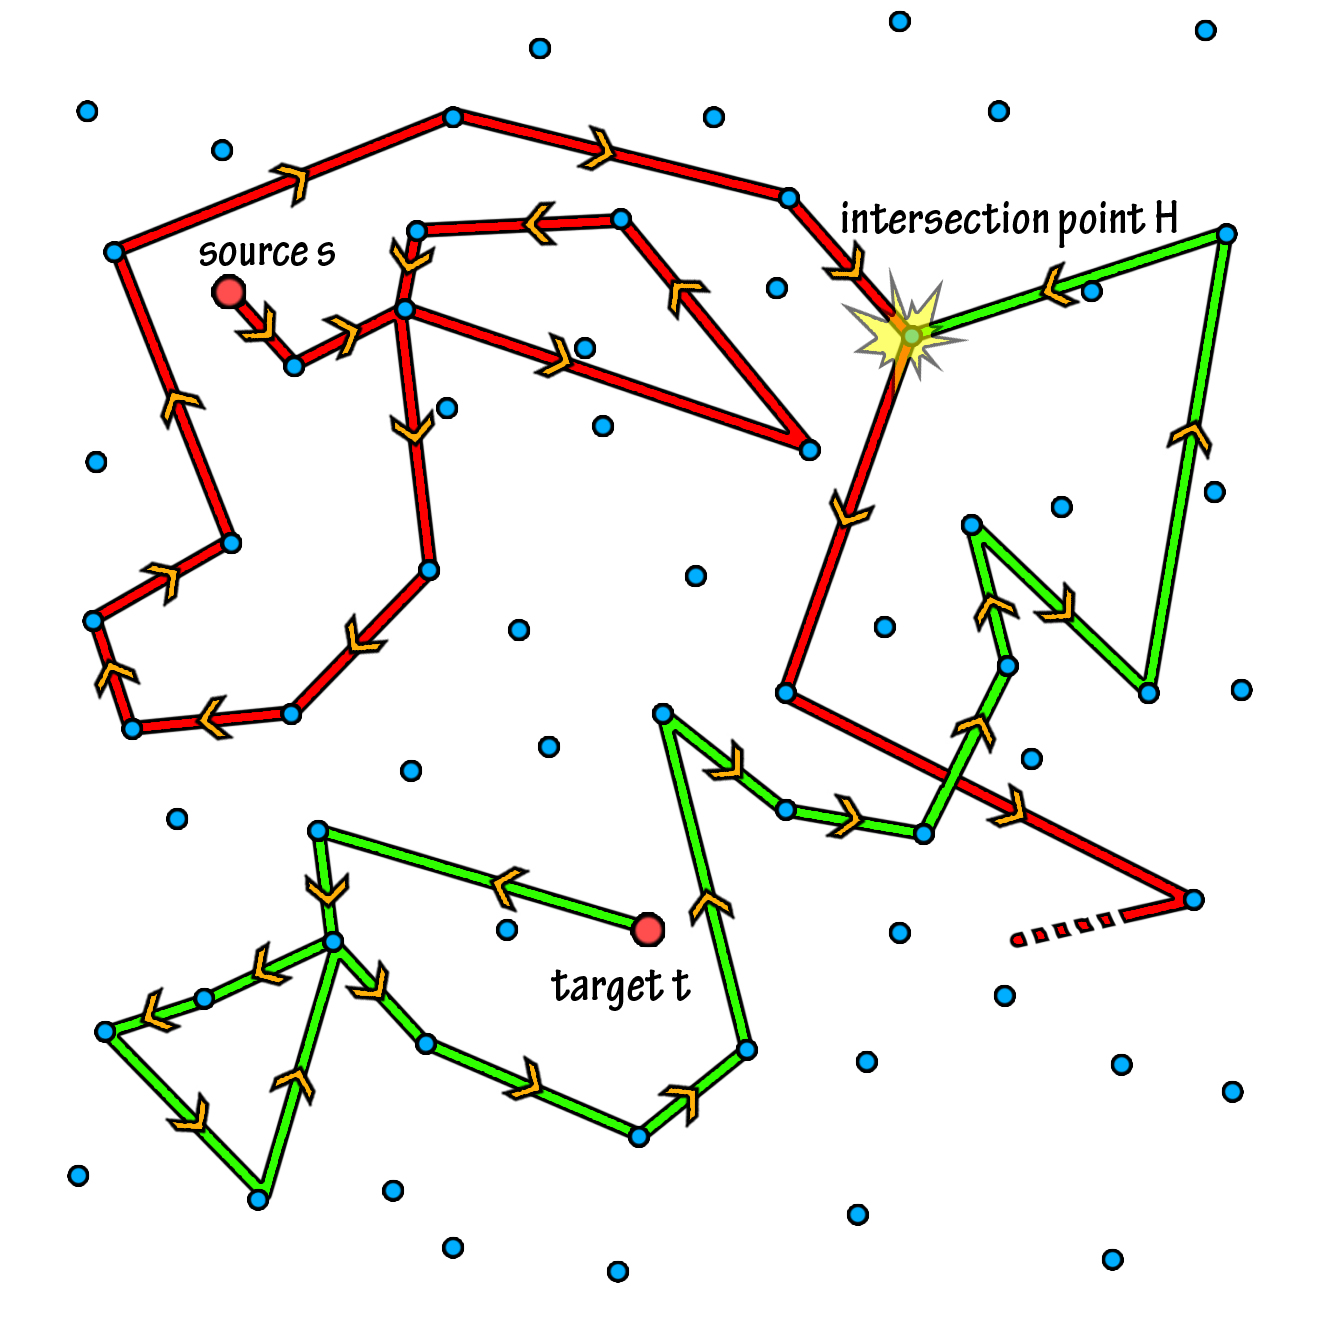
\includegraphics[scale=0.15]{Results/2rawrandomwalk.jpg}
\caption{2-Way Random Walk}
\label{4_two_way}
\end{figure}


\subsection{The Measure of Performance}
The measure of performance of any algorithm forms an important part of its analysis. The performance of our algorithm is measured on a relative scale.  We choose the following parameters as performance measures.
\begin{itemize}
	\item Running Time: \\
	The time required for an algorithm to execute forms an important factor to measure performance. In this study, we empirically compare the running time of our algorithm with that of unidirectional Adamic technique. Note that, for a given pair of nodes, we have run both the algorithms under similar computing environments. This eliminates the effects that the computing environments pose towards the performance of the algorithm.
	
	\item Average value of $\frac{actual\ path\ length }{shortest\ path\ length}$: \\
	The fraction $\frac{path\ length }{shortest\ path\ length}$ denotes the factor by which the path length obtained by our algorithm is greater than the actual shortest path length. We consider the average of this value over a large number of randomly chosen node pairs.
	
	\item Performance factor $\frac{1}{time*average \frac{path\ length}{shortest\ path\ length}}$: \\
	The performance of the algorithm is said to be high if it produces a shorter path and takes a relatively lesser amount of time. Assuming that the performance varies inversely as the parameters mentioned above, we empirically consider this fraction as an effective performance measure.
\end{itemize}

\subsection{Subtle issues involving constraints and decision logic}
The implementation of an algorithm reveals its subtleties. Many issues / design decisions come into light only when we implement the algorithms. In this section, we present the subtleties and optimizations that has been brought about during the implementation of the algorithm.
\begin{enumerate}
\item Parallelization: \\
A parallel algorithm is an algorithm that can be executed one piece at a time on many different processing devices. The results from individual processing threads are then combined back into one single result. All the algorithms cannot be divided into parallel pieces. It is the inherent nature of the algorithm which makes it parallelizable.\\

The core step of our algorithm is the advancements that the walkers make at each time step. Since either of the walkers do not influence the hop decision of the other walker, our algorithm can be \emph{theoritically} parallelized. Although this may sound theoretically feasible, the practical implementation poses a variety of problems. One such example is presented below.\\
%granularity

Let A and B be two threads running in parallel. Note that the threads are running in parallel, not simultaneously. The interleaving period for each thread is sufficient for one of the walkers to race past the other. Ideally, each walker must take turns in advancing a single step. This leads to a race condition. Consider a snippet of the actual scenario shown below. \\
$Path_A: ['24', '3', '23']$\\
$Path_B ['26', '4', '23', '12', '7', '12', '9', '4', '18', '3']$\\
Intersection Point: '3'\\
This lack of synchronization leads to the wrong choice of the intersection point, thereby increasing the effective path length.

\item Formation of Cycles\\
On an abstract level, unidirectional Adamic walk suggests that the next hop should be made to the neighbor with the highest degree. Trivially, the idea seems to be functional in all the cases. Further analysis reveals that such a step leads to the formation of cycles. If a walker hops to the richest neighbor and causes a cycle formation, it can never exit the cycle. This causes the walker to stay on the cycle for eternity. To avoid such a scenario, Adamic suggested that the walker should hop on to the neighbor with the next highest degree in case a cycle formation is detected in prior.\\

In this design decision, our algorithm differs from that of Adamic's. The computational cost (time) involved in deducing the neighbor with the next highest degree is relatively high. Hence, we make a random choice for next hop.\\

This solution works with a very high probability. But there are situations wherein a hop to any of the neighbors would lead to the formation of a cycle. In other words, the walker would have already visited all the neighbors. In such a case, we suggest to take 2 random hops. Ofcourse, this causes a cycle, but the difference is that the walker is not placed within the cycle. This allows the walker to continue its quest for the intersection point.\\

\item Performance Optimization - Flagging technique instead of Linear Search\\
A trivial algorithm for identifying the formation of cycles in the network is to search whether the next node is already in the path traversed by the walker. This requires a linear traversal through the list that represents the path. The formation of cycles must be checked before every hop. This leads to a high degree of complexity. A more efficient way to handle this scenario is to flag the nodes that have already been visited. Before every hop, the flag is checked. If the flag is set, it indicates that the node has been visited, thus leading to the formation of a cycle. If the flag is not set, the hop is made and the flag is set.
\end{enumerate}

\section{Application of our algorithm to various classes of networks}
In the subsections below, we present and discuss four results for Erdos-Renyi Graphs and Barabasi-Albert Network. The first figure depicts a comparison of the average $\frac{length of actual path}{length of shortest path}$ between two-way random walk and two-way adamic walk, for varying number of nodes. The second figure compares the relative time taken by one-way adamic walk and two-way adamic walk, for varying number of nodes. The third figure compares the average $\frac{length of actual path}{length of shortest path}$ for one-way random walk, two-way random walk, one-way adamic walk and two-way adamic walk. The fourth figure depicts the variation of the performance measure that we had defined earlier - $\frac{1}{time*average \frac{path\ length}{shortest\ path\ length}}$ for all the four methods, with varying number of nodes.

\subsection{Application of the algorithm on Erdos-Renyi Graphs}
In this section, we present the results obtained when our algorithm was applied to a class of networks known as Erdos Renyi networks. An Erdos Renyi network G(n,p) is a random graph obtained by starting with n vertices and adding edges between them at random with a probability p. The experiments were conducted for varying number of nodes in a graph, keeping the attachment probability $p$ as $0.3$. The following figures show the results obtained from our experiments.

\begin{figure}[htp]
\centering
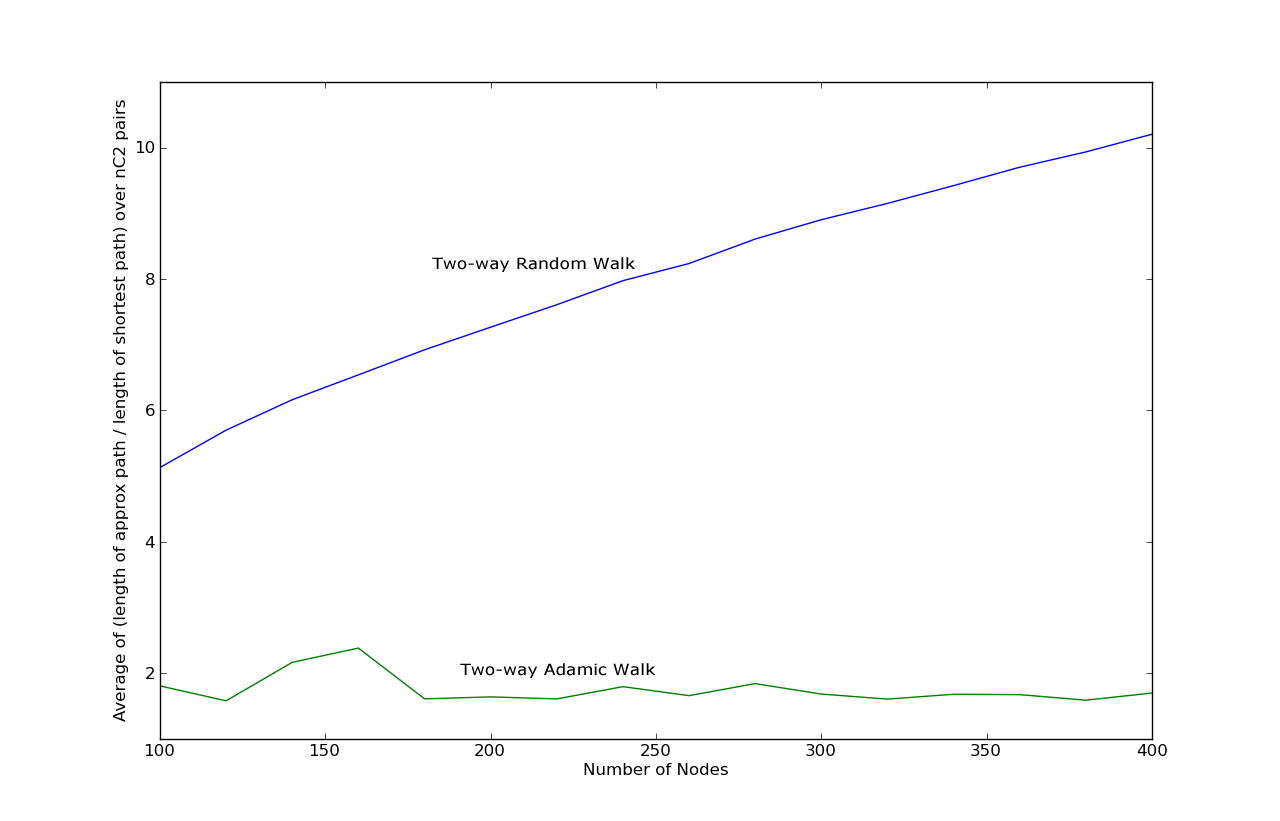
\includegraphics[scale=0.40]{Results/ERratio2Random2Adamic.png}
\caption{average $\frac{length of actual path}{length of shortest path}$ for Erdos Renyi Networks}
\label{ERratio2Random2Adamic}
\end{figure}
This plot shows the variation of average $\frac{length of actual path}{length of shortest path}$ for Two-way Random walk and Two-way Adamic walk. The algorithm has been tested on Erdos Renyi graphs with 0.3 probability and the number of nodes varying from between 100 to 400. The length of the path obtained Two-way adamic walk is around 1.75 times the shortest path length, on an average. As the number of nodes increase, the average value of $\frac{length of actual path}{length of shortest path}$ increases for the Two-way Random walk technique. Our proposed method is almost an invariant with respect to the number of nodes. 

\newpage
\begin{figure}[htp]
\centering
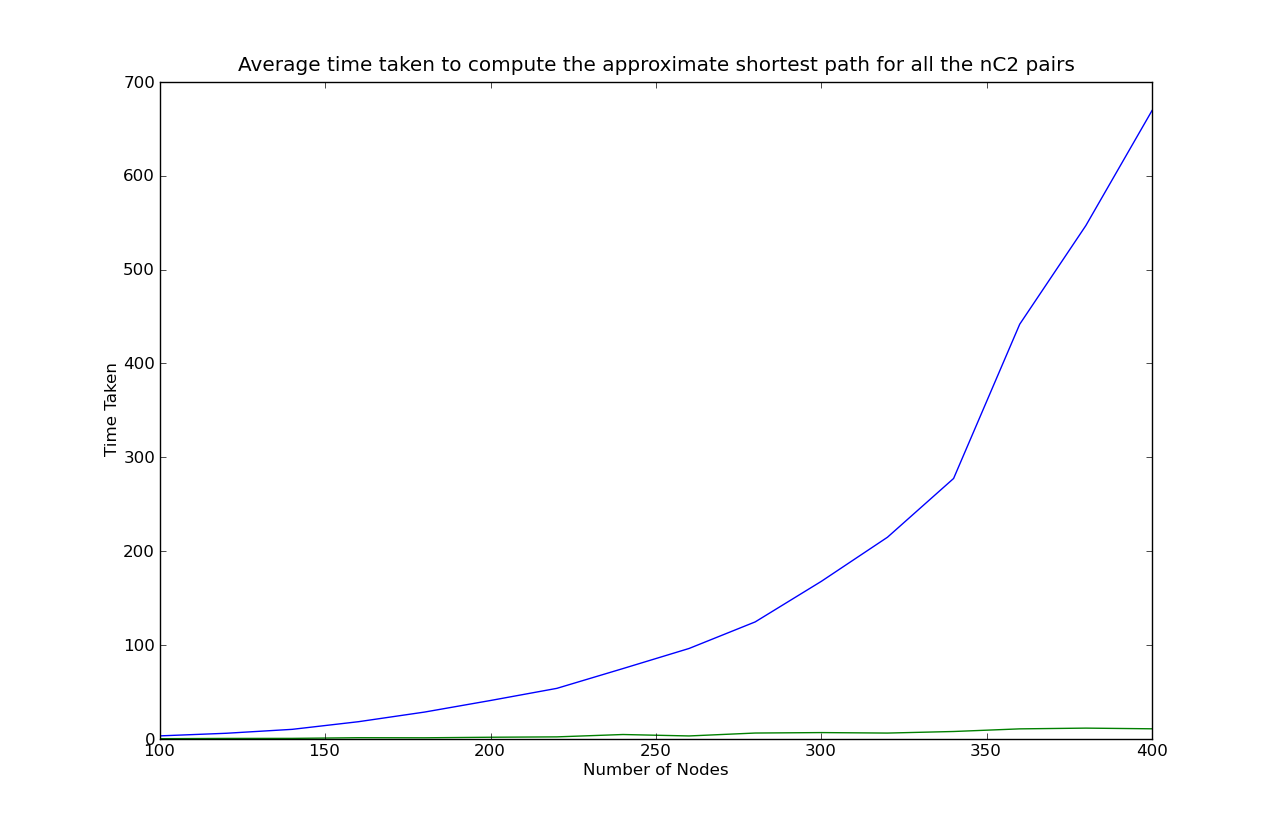
\includegraphics[scale=0.40]{Results/ERtime1Adamicand2Adamic.png}
\caption{Time Taken}
\label{ERtime1Adamicand2Adamic}
\end{figure}
This plot shows the variation of the average time taken to establish connection between arbitrary pair of nodes in an Erdos Renyi network. This figure depicts the contrast between the connection establishment time using one-way adamic walk and two-way adamic walk. As seen from the figure, the connection establishment time exponentially increases in the case of one-way Adamic walk.

\begin{figure}[htp]
\centering
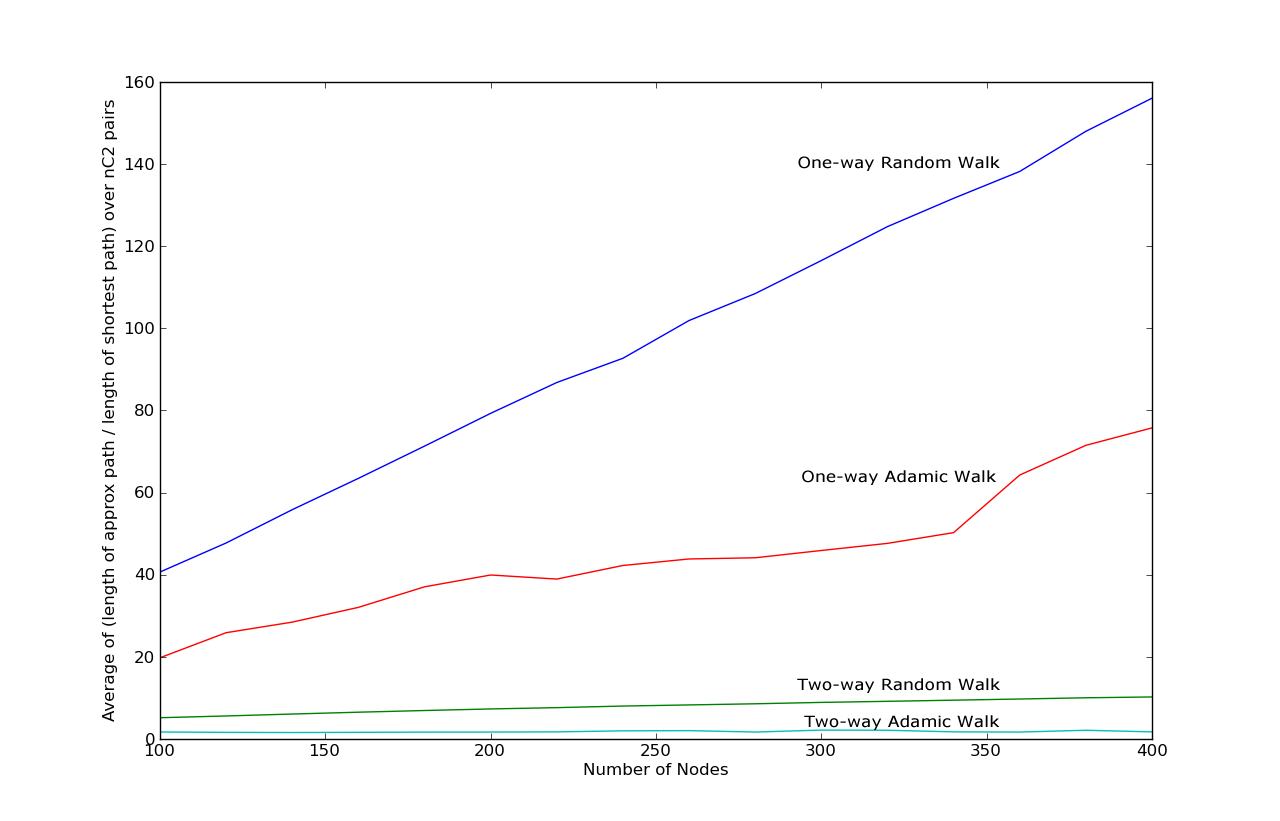
\includegraphics[scale=0.40]{Results/ERratioall.png}
\caption{average $\frac{length of actual path}{length of shortest path}$ for Erdos Renyi Graph with 0.3 probability}
\label{ERratio-all}
\end{figure}
This plot shows the variation of average $\frac{length of actual path}{length of shortest path}$ for One-way Random walk, Two-way Random walk One-way Adamic walk and Two-way Adamic walk.

\newpage
\begin{figure}[htp]
\centering
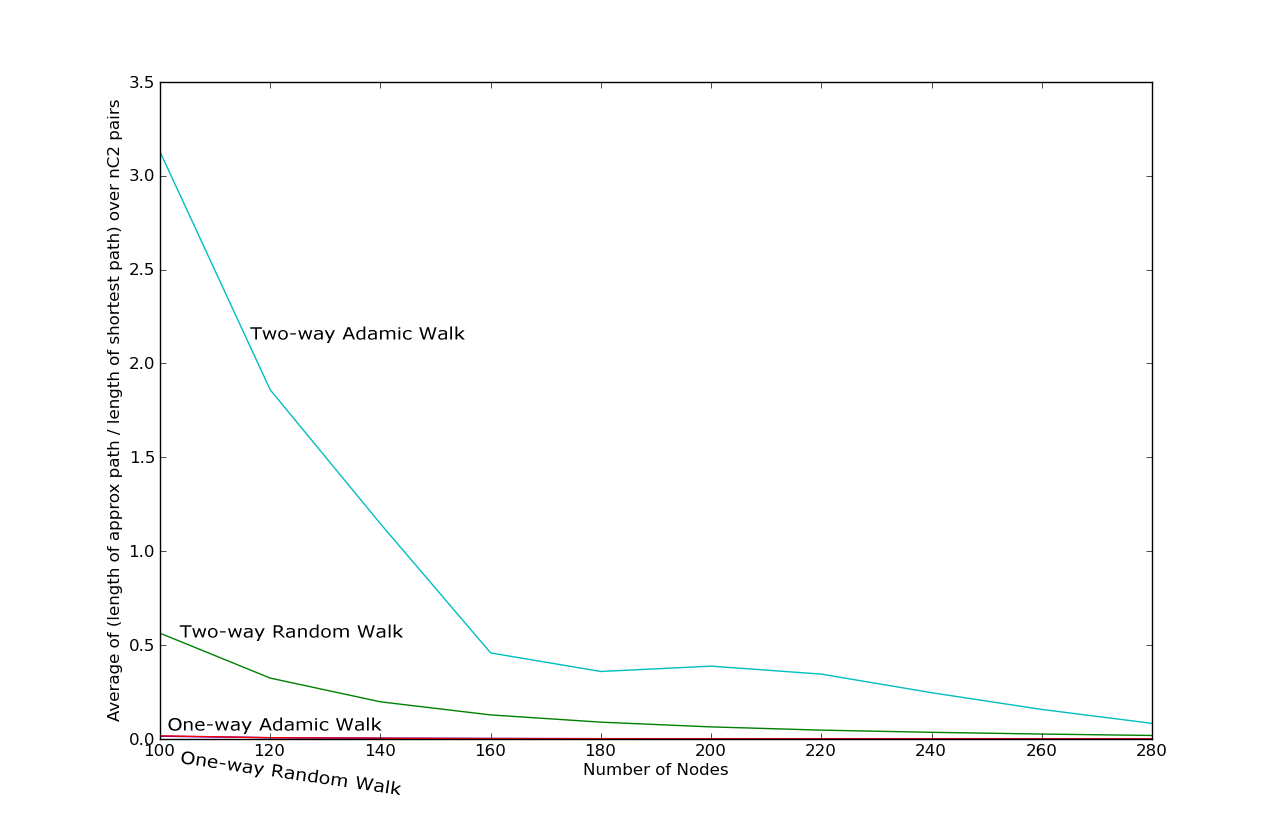
\includegraphics[scale=0.40]{Results/ERperformance.png}
\caption{average $\frac{length of actual path}{length of shortest path}$ for Erdos Renyi Networks}
\label{ERperformance}
\end{figure}
The performance measure that we introduced earlier is plotted against the varying number of nodes for an Erdos Renyi Network. As expected, the performance of the two-way adamic walk better than the other methods. But the performance factor decreases as number of nodes increases. This is probably due to the fact that the formula was chosen empirically.




\subsection{Application of the algorithm on Barabasi Albert Networks}

\begin{figure}[htp]
\centering
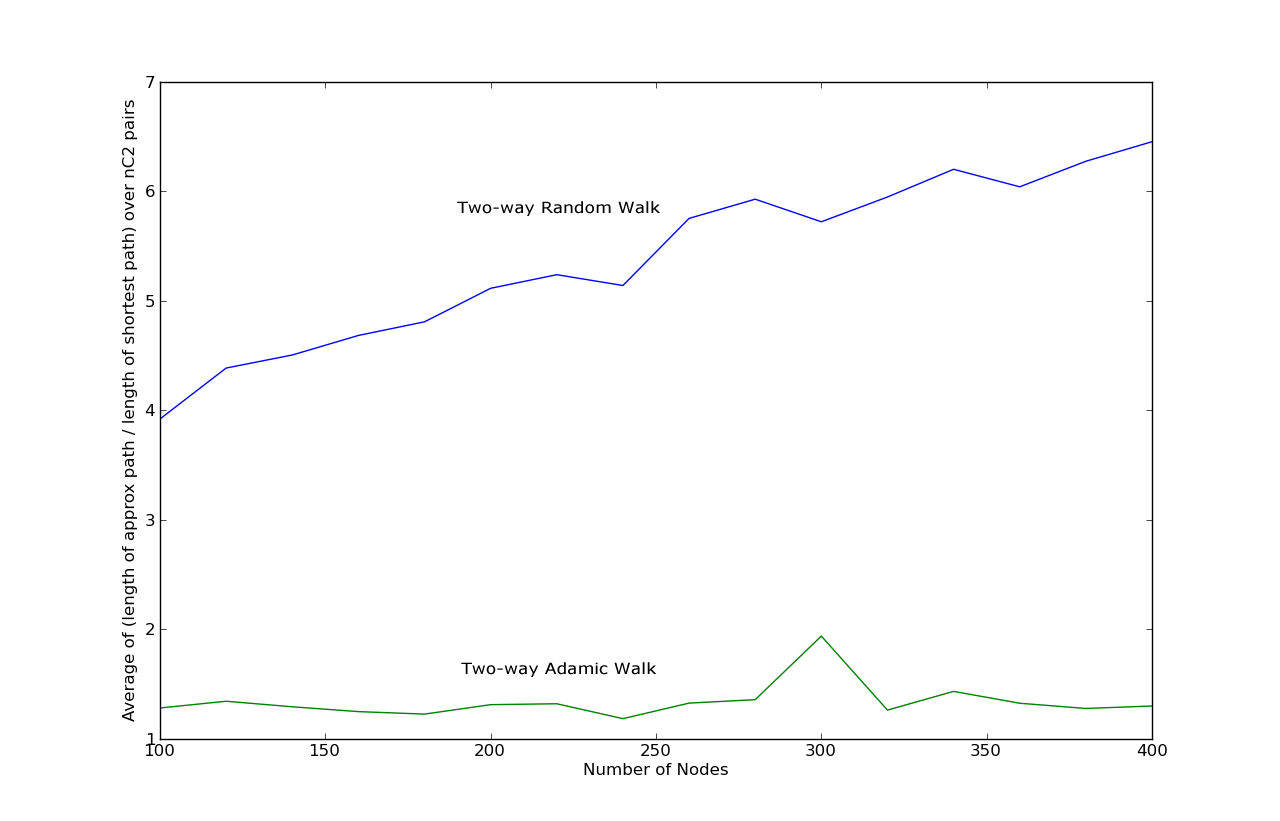
\includegraphics[scale=0.40]{Results/SFNratio2Random2Adamic.png}
\caption{average $\frac{length of actual path}{length of shortest path}$ for Barabasi Albert Network of degree 3}
\label{SFNratio2Random2Adamic}
\end{figure}
This plot shows the variation of average $\frac{length of actual path}{length of shortest path}$ for Two-way Random walk and Two-way Adamic walk. The algorithm has been tested on Barabasi Albert Networks with degree 3 and the number of nodes varying from between 100 to 400. The length of the path obtained Two-way adamic walk is around 1.25 times the shortest path length, on an average. Clearly, The average in the case of Power Law Networks is smaller than that of Erdos Renyi Networks. As the number of nodes increase, the average value of $\frac{length of actual path}{length of shortest path}$ increases for the Two-way Random walk technique. Our proposed method is almost an invariant with respect to the number of nodes. 

\begin{figure}[htp]
\centering
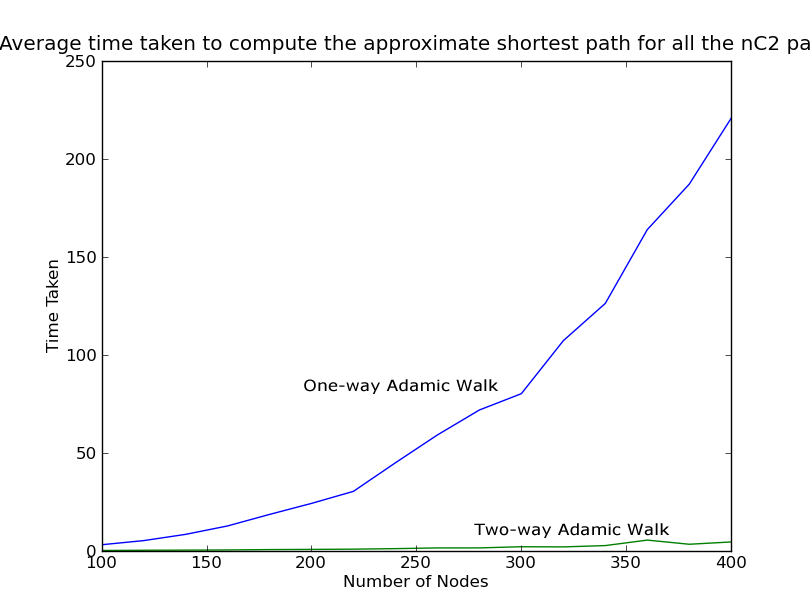
\includegraphics[scale=0.50]{Results/SFNtime1Adamicand2Adamic.png}
\caption{Time Taken}
\label{SFNtime1Adamicand2Adamic}
\end{figure}
This plot shows the variation of the average time taken to establish connection between arbitrary pair of nodes in a Barabasi Albert network. This figure depicts the contrast between the connection establishment time using one-way adamic walk and two-way adamic walk. As seen from the figure, the connection establishment time exponentially increases in the case of one-way Adamic walk.

\begin{figure}[htp]
\centering
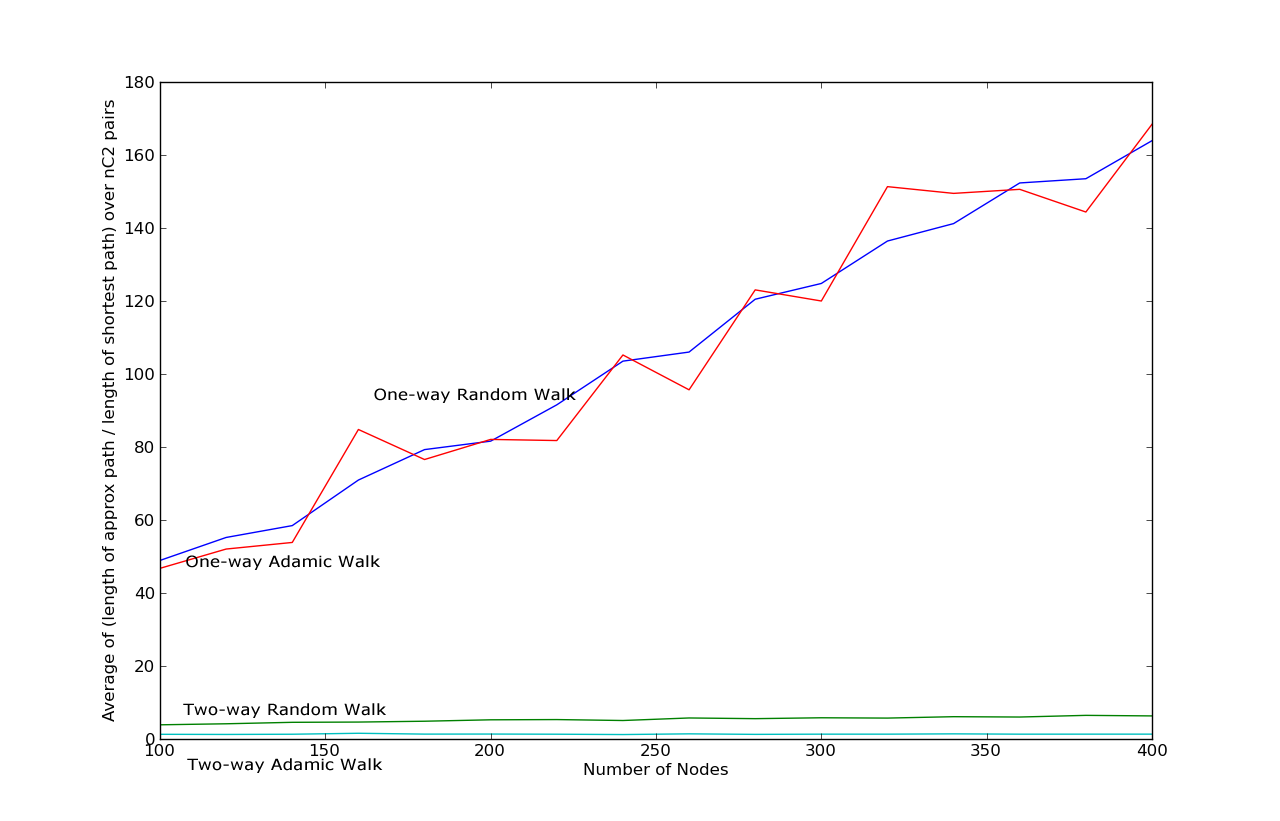
\includegraphics[scale=0.40]{Results/SFNratioall.png}
\caption{average $\frac{length of actual path}{length of shortest path}$ for Barabasi Albert Network of degree 3}
\label{SFNratio-all}
\end{figure}
This plot shows the variation of average $\frac{length of actual path}{length of shortest path}$ for One-way Random walk, Two-way Random walk One-way Adamic walk and Two-way Adamic walk. The performance of One-way Random walk and One-way Adamic walks are comparable. The performance of One-way Random walk is as expected. The One-way adamic walk fails to perform well because the nodes in the periphery are hard to reach using Adamic's technique. Hence, it is comparable to a One-way Random walk.

\begin{figure}[htp]
\centering
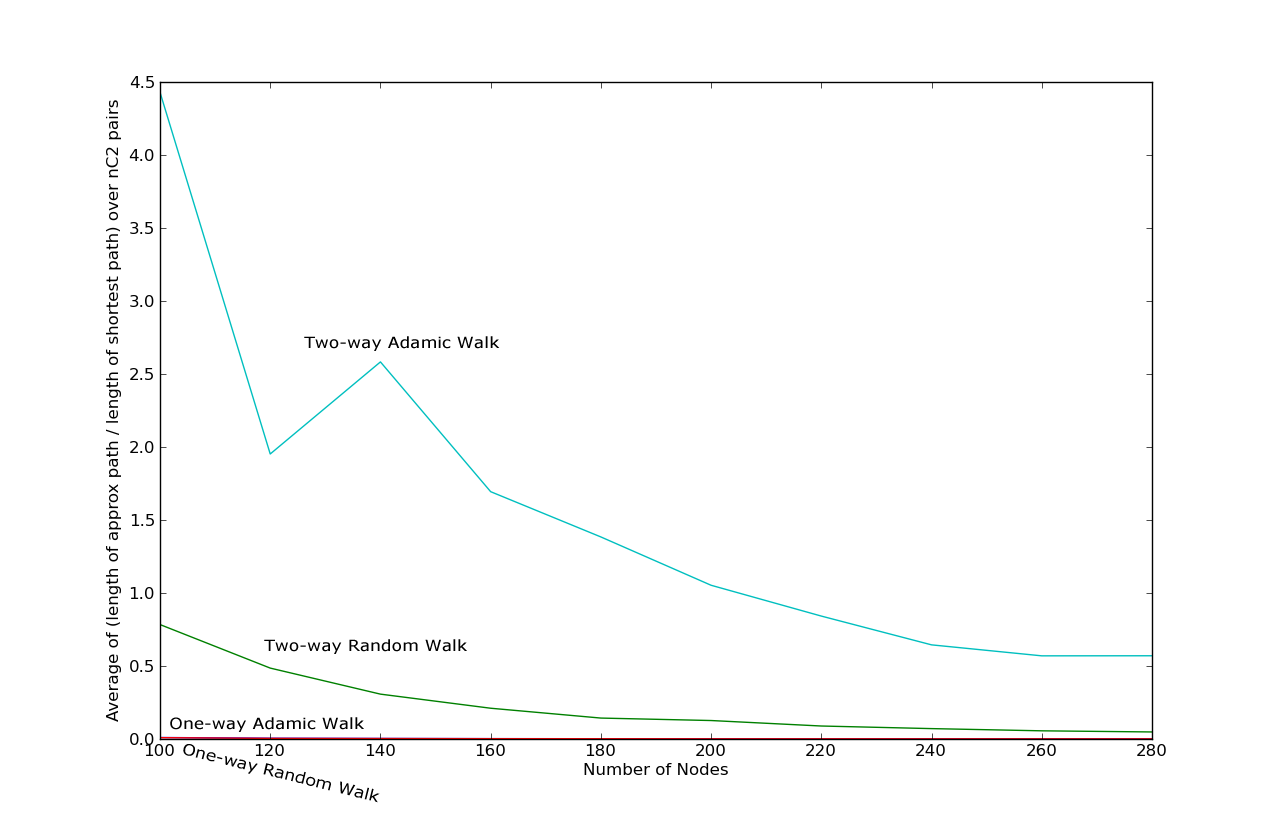
\includegraphics[scale=0.30]{Results/SFNperformance.png}
\caption{average $\frac{length of actual path}{length of shortest path}$ for Barabasi Albert Network of degree 3}
\label{SFNperformance}
\end{figure}
The performance measure that we introduced earlier is plotted against the varying number of nodes for a Barabasi Albert Network. As expected, the performance of the two-way adamic walk better than the other methods. But the performance factor decreases as number of nodes increases. This is probably due to the fact that the formula was chosen empirically.


\subsection{Application of the algorithm on Gnutella network}
Gnutella is a system in which individuals can exchange files over the Internet directly without going through a Web site. This is achieved using a peer-to-peer arrangement. In our experiments, we consider the gnutella network provided at\\ http://snap.stanford.edu/data/p2p-Gnutella08.html. A sequence of snapshots of the Gnutella peer-to-peer file sharing network had been sampled during August 2002. There are total of 9 snapshots of Gnutella network collected in August 2002. Nodes represent hosts in the Gnutella network topology and edges represent connections between the Gnutella hosts. We consider the sample taken on 8th August 2002. The degree distribution of the considered gnutella network is shown in the figure ~\ref{gnutellaNetwork}. Clearly, the network exhibits Scale Free behavior.\\

\begin{figure}[htp]
\centering
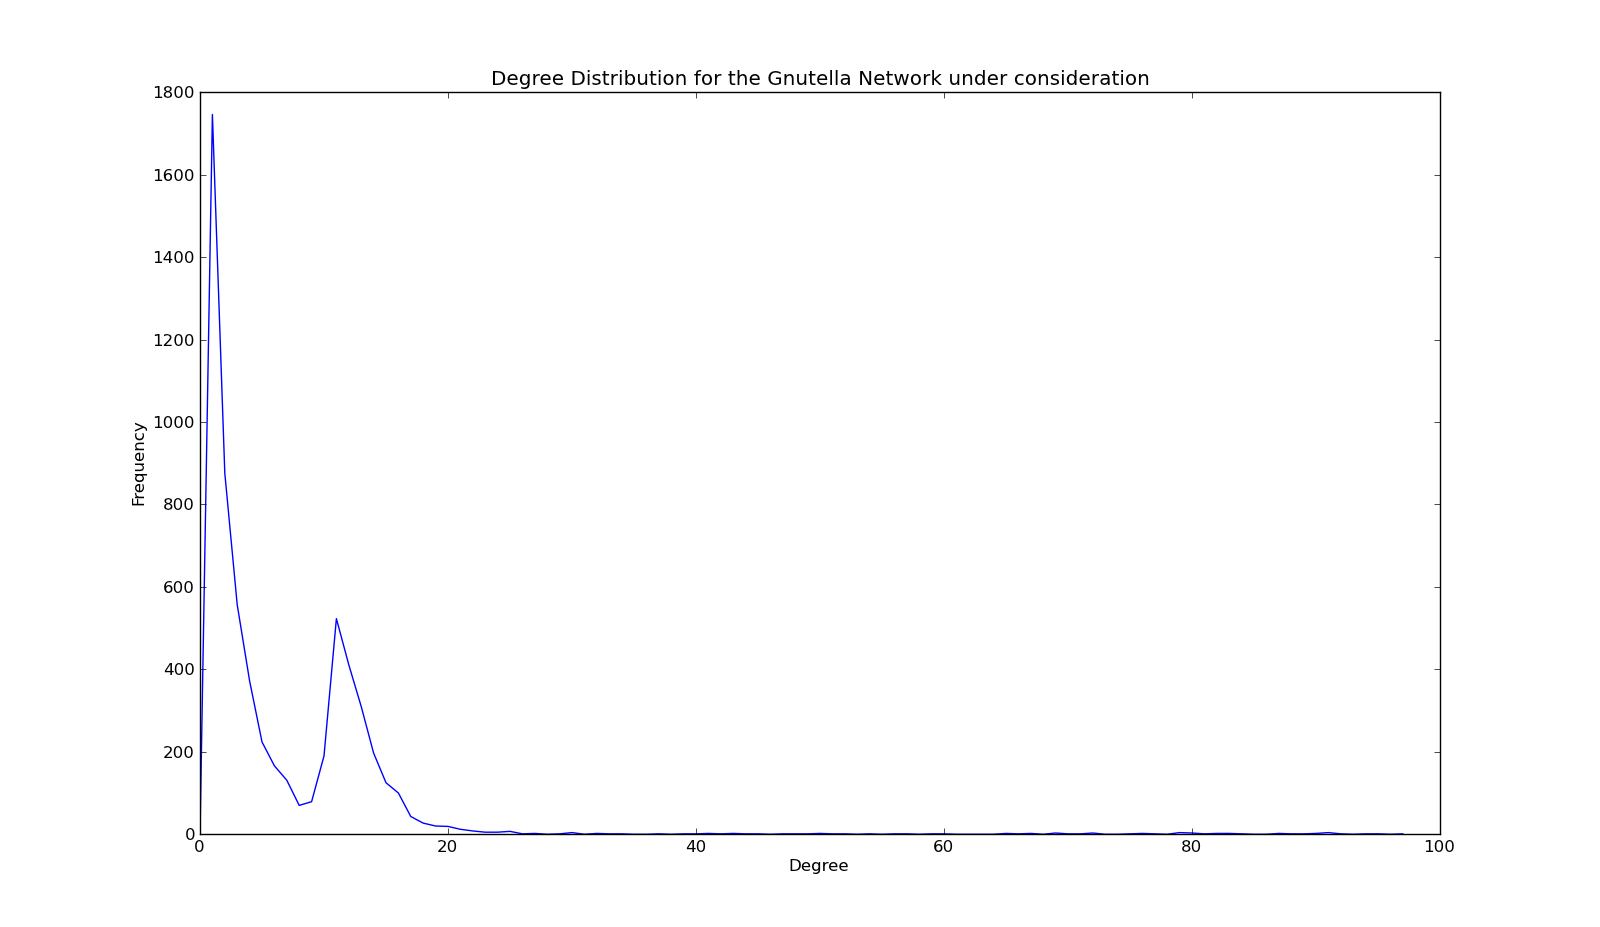
\includegraphics[scale=0.3]{Results/gnutellaNetwork.png}
\caption{Scale Free Nature of the considered gnutella network}
\label{gnutellaNetwork}
\end{figure}

We make 2 important assumptions for our algorithm to be applied for the dataset. First, we convert the directed edges of the network into undirected edges to indicate the bidirectional data transfer. Second, we consider the largest connected subgraph from the given dataset. We observe that two of the nodes are disconnected in the given dataset. Hence, we consider an undirected connected subgraph of the gnutella network consisting of 6299 nodes and 20776 edges. For each experiment, 5000 node pairs are picked at random and the algorithms are applied for comparison. The following figures depict the results obtained.

\newpage

\begin{figure}[htp]
\centering
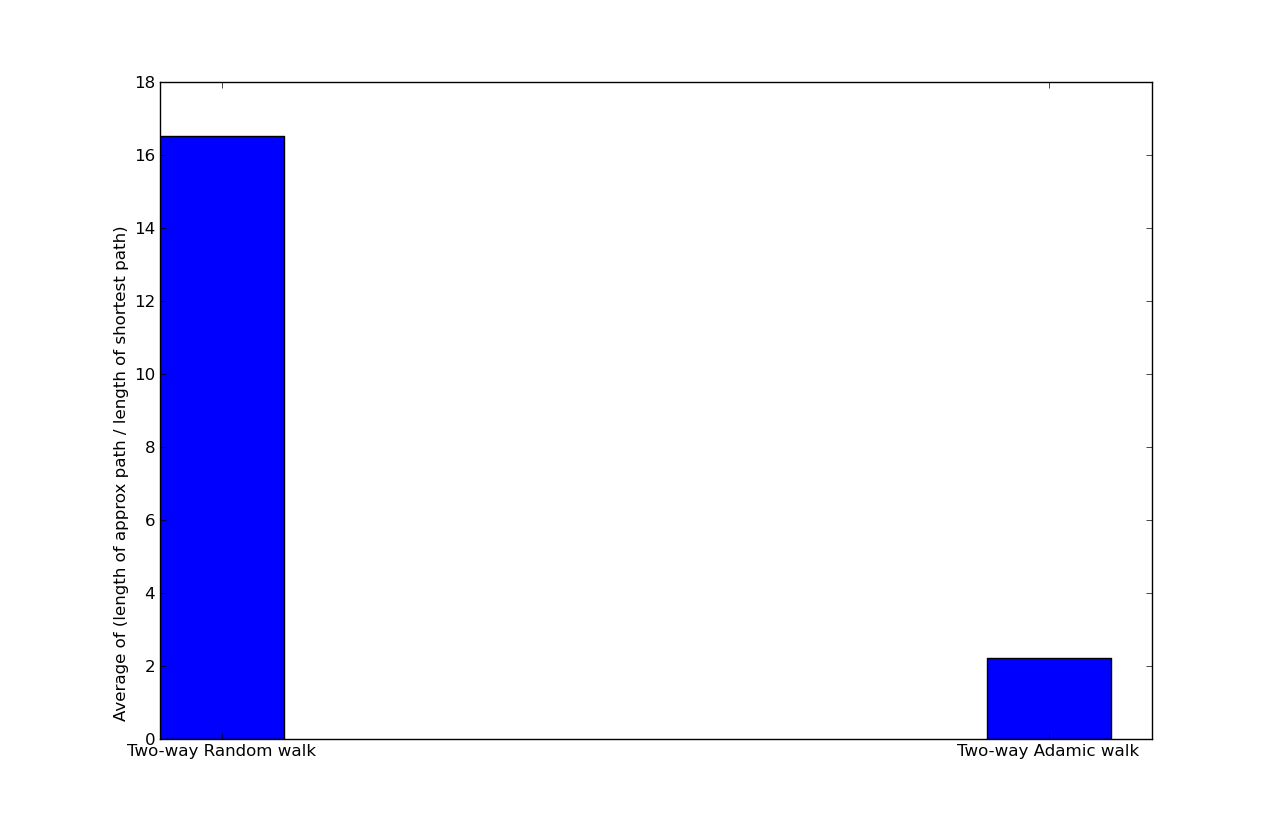
\includegraphics[scale=0.45]{Results/gnutellaAvrgPath.png}
\caption{average $\frac{length of actual path}{length of shortest path}$ for a gnutella network consisting of 6299 nodes and 20776 edges}
\label{gnuAvrgPath}
\end{figure}
The above figure shows the average time required to establish connection between a randomly chosen pair of nodes in the considered gnutella network. Clearly, the average ratio of $\frac{length of actual path}{length of shortest path}$ using two-way random walk technique exceeds the average ratio using two-way Adamic walk by a large factor. The Two-way random technique yields a ratio of approximately 16, while the Two-way Adamic walk yields a ratio of approximately 2. This shows that the connection can be established in the gnutella network using Two-way Adamic walk is much shorter, relative to the path obtained using Two-way Random walk.

\newpage
\begin{figure}[htp]
\centering
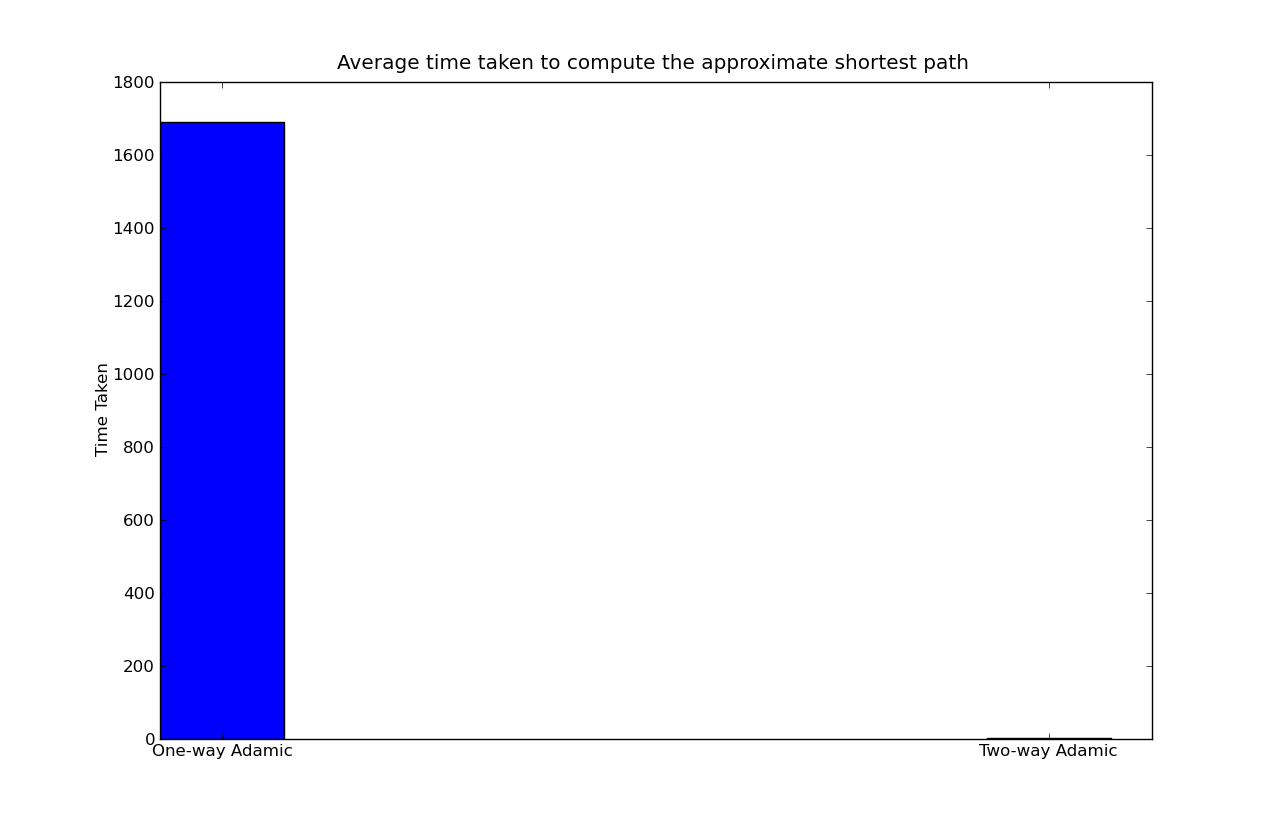
\includegraphics[scale=0.45]{Results/gnutellaTimePlot.png}
\caption{average $\frac{length of actual path}{length of shortest path}$ for a gnutella network consisting of 6299 nodes and 20776 edges}
\label{gnuTime}
\end{figure}
The above figure shows the average time required to establish connection between a randomly chosen pair of nodes in the considered gnutella network. Clearly, the average time required to establish connection using One-way Adamic walk is far larger than the time taken using Two-way Adamic walk. The ratio of the time intervals taken to perform One-way Adamic walk and Two-way Adamic walk is 524.062. Hence, Two-way Adamic walk is faster than One-way Adamic walk by a factor of 0.001908169, on the considered gnutella network.

\section{Implementation}
\begin{itemize}
 \item The above algorithm has been implemented using Python 2.7. 
 \item Python Development Kits used :
 \begin{itemize}
  \item NetworkX
  \item Matplotlib
  \item Numpy
  \item Scipy
  \item Pickle  
  \item Random
 \end{itemize}
\item yEd network visualization tool from yWorks.
\\\emph{http://www.yworks.com/en/products\_yed\_download.html}
\end{itemize}

\section{Conclusion}
\label{sec:4_conclusion}
Motivated by the strategy adopted by humans to navigate in an unknown environment and the One-way Adamic graph navigation technique, we presented in this study, an extension to the algorithm proposed by Adamic. We showed that the algorithm performs better than the One-way Random walk, Two-way Random walk and One-way Adamic walk techniques on Power Law Networks.\\

A possible further work would be to formulate the thoeritical complexity and bounds of the algorithm. It would be interesting to compare our algorithm with the complexities of other navigational techniques. It would also be interesting to classify the networks on which the algorithm performs well and those on which it does not.

\bibliographystyle{plain}
\bibliography{references}

\end{document}